\documentclass{article}

%Basics
\usepackage[margin=1in]{geometry}
\usepackage{amsmath, amssymb, amsthm}
\usepackage{enumitem}

%Vertical Dots in Align Environment
\usepackage{mathtools}

%Creating Figures
\usepackage{tikz}
\usetikzlibrary{calc, math, matrix, graphs, positioning}

%Subfigures
\usepackage{subcaption}

%Multiple Columns
\usepackage{multicol}

%Formatting and Spacing
\setitemize[1]{noitemsep, parsep = 5pt, topsep = 5pt}
\setenumerate[1]{label = (\alph*), parsep = 1pt, topsep = 5pt}
\setlength\parindent{0pt}
\linespread{1.1}

%Easy Numbering
\newcounter{counter}
\newcommand{\Exercise}{Exercise \stepcounter{counter}\thecounter}

%Cases Environment
\newlist{Cases}{enumerate}{3}
\setlist[Cases]{leftmargin = .25in, label = {Case \arabic*.}, topsep = 0.01in, itemsep = 0.04in, itemindent = .5in, parsep = 0in}

%Custom Title Fields
\newcommand{\hmwkTitle}{Homework 5 (with Solutions)}
\newcommand{\hmwkDueDate}{March 12, 2022}
\newcommand{\hmwkClass}{Honors Discrete Mathematics}
\newcommand{\hmwkClassInstructor}{Gerandy Brito}
\newcommand{\hmwkSection}{Spring 2022}
\newcommand{\hmwkAuthorName}{Sarthak Mohanty}

%Headers and Footers
\usepackage{fancyhdr}
\usepackage{extramarks}
\pagestyle{fancy}
\lhead{\hmwkAuthorName}
\chead{\hmwkClass \ (\hmwkClassInstructor)}
\rhead{Homework 5}
\cfoot{\thepage}
\renewcommand\headrulewidth{0.4pt}
\renewcommand\footrulewidth{0.4pt}

\title{
    \vspace{2in}
    \textbf{\hmwkClass:\\ \hmwkTitle}\\
    \normalsize\vspace{0.1in}\small{Due\ on\ \hmwkDueDate\ at 11:59pm}\\
    \vspace{0.1in}\large{\textit{\hmwkClassInstructor\ \hmwkSection}}
    \vspace{3in}
    \author{\textbf{\hmwkAuthorName}}
    \date{}
}

\begin{document}

\maketitle
\pagebreak

\subsection*{\Exercise}
    Define a relation $\le_{i}$ on the Cartesian product $A_{1} \times A_{2} \times \cdots \times A_{n}$ as such: Given two sequences $(a_{n}) = (a_{1}, a_{2}, \dots, a_{n})$ and $(b_{n}) = (b_{1}, b_{2}, \dots, b_{n})$, declare that $(a_{n}) \le_{i} (b_{n})$ if and only if $a_{i} \le b_{i}$ for all $1 \le i \le n$.
    \begin{enumerate}
        \item Prove that this relation is a partial order.
        \item Let $Z = \{-3, -2, -1, 0, 1, 2, 3\}$. Draw a Hasse diagram corresponding to the poset $(Z \times Z, \le_{i})$. Briefly explain the general structure of this diagram if we were to extend the domain to all $\mathbb{Z} \times \mathbb{Z}$, and its similarity to the Cartesian plane.
        \item If we define this relation on the Cartesian product of $n$ totally ordered sets, is the relation a total order? Either prove or provide a counterexample.
    \end{enumerate}

\subsection*{Solution}
    \begin{enumerate}
        \item This relation is a partial order if it is reflexive, antisymmetric, and transitive. For all $(a_{n}), (b_{n}), (c_{n}) \in A$, we have
        \begin{enumerate}[label = \arabic*.]
            \item \textit{(Reflexivity)} $a_{i} \le a_{i}$ for all $i$, so $(a_{n}) \le (a_{n})$.
            \item \textit{(Antisymmetry)} Suppose $(a_{n}) \le_{i} (b_{n})$ and $(b_{n}) \le_{i} (a_{n})$. Then $a_{i} \le b_{i}$ and $b_{i} \le a_{i}$ for all $i$, so $a_{i} = b_{i}$ for all $i$. Thus $(a_{n}) = (b_{n})$.
            \item \textit{(Transitivity)} Suppose $(a_{n}) \le_{i} (b_{n})$ and $(b_{n}) \le_{i} (c_{n})$. Then $a_{i} \le b_{i}$ and $b_{i} \le c_{i}$ for all $i$, so $a_{i} \le c_{i}$ for all $i$, so $(a_{n}) \le_{i} (c_{n})$.
        \end{enumerate}
        \item For the Hasse diagram, see Figure \ref{fig:Q1}. If we extend the domain to all $\mathbb{Z} \times \mathbb{Z}$, the diagram becomes a $45^{\circ}$ rotation of the Cartesian plane. 
        
        \vspace{1.5mm}
        \textbf{Remark:} Distances and angles do not necessarily need to be preserved in the Hasse Diagram, so there may be different interpretations.
        \item No. $\mathbb{N}$ is totally ordered, but over $\mathbb{N} \times \mathbb{N}$, the two ordered pairs $(0, 1)$ and $(1, 0)$ are not comparable.
    \end{enumerate}

    \begin{figure}[htbp]
        \centering
        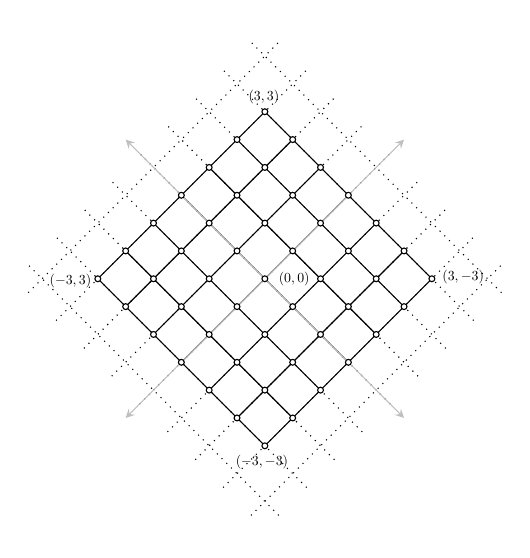
\begin{tikzpicture}[rotate=45, scale = .5, circ/.style={shape=circle, draw, node contents= {}, fill = white}, inner sep=1.5pt, transform shape]
            \draw[dotted] (-4.5,-4.5) grid (4.5,4.5);
            \draw (-3, -3) grid (3,3);
            \draw[stealth-stealth, gray!50] (-5,0)--(5,0) node[right]{};
            \draw[stealth-stealth, gray!50] (0,-5)--(0,5) node[above]{};
            \foreach \x in {-3, -2, -1, 0, 1, 2, 3}
                  \foreach \y in {-3, -2, -1, 0, 1, 2, 3}
                    \draw node at (\x, \y) [circ];
            %Coordinate Bashing
            \draw node at (0, 0) [yshift = -15pt, xshift = 15pt] { \rotatebox{-45}{$(0, 0)$}};
            \draw node at (-3, -3) [yshift = -7pt, xshift = -10pt] {\rotatebox{-45}{$(-3, -3)$}};
            \draw node at (-3, 3) [yshift = 13pt, xshift = -15pt] {\rotatebox{-45}{$(-3, 3)$}};
            \draw node at (3, -3) [yshift = -15pt, xshift = 17pt] {\rotatebox{-45}{$(3, -3)$}};
            \draw node at (3, 3) [yshift = 8pt, xshift = 7pt] {\rotatebox{-45}{$(3, 3)$}};
        \end{tikzpicture}
        \caption{Hasse diagram of the poset $(Z \times Z, \le_{i})$.}
        \label{fig:Q1}
    \end{figure}

\subsection*{\Exercise}
   \begin{enumerate}
       \item Draw the Hasse diagram of the poset $(D_{2470}, \mid)$, where $D_{n}$ is the set of all positive integers that divide $n$, and $\mid$ is the divisibility relation.
       \item Draw the Hasse diagram of the poset $(\mathcal{P}(\{2, 5, 19, 13\}), \subseteq)$. Explain the similarities between this Hasse diagram and the Hasse diagram in part (a), and the underlying relationship between the two posets causing these similarities.
       \item Without explicitly drawing the diagrams, explain the similarities between the Hasse diagrams of the posets $(D_{140}, \mid)$ and $(D_{525}, \mid)$, and the underlying relationship between the two posets causing these similarities.
       
       \vspace{1.5mm}
       \textit{Hint:} Consider using a similar (but not identical!) argument as in part (b).
   \end{enumerate}

\subsection*{Solution}
    \begin{enumerate}
        \item For the Hasse diagram, see Figure \ref{fig:Q2a}.
        \item For the Hasse diagram, see Figure \ref{fig:Q2b}. There is a one-to-one correspondence (bijection) between the elements of the Hasse diagram in part (a) and the elements of the Hasse diagram in part (b). This occurs because $2470 = 2 \cdot 5 \cdot 13 \cdot 19$, and any divisor of $2470$ is the product of the elements in exactly one subset of the set containing this prime factorization.
        
        \vspace{1.5mm}
        \textbf{Remark}: Posets having Hasse Diagrams with this type of relationship are known as \textit{order isomorphic}.
        \item $140$ has the prime factorization $2^{2} \cdot 5^{1} \cdot 7^{1}$, while $525$ has the prime factorization $3^{1} \cdot 5^{2} \cdot 7^{1}$. We now define the two posets $(\mathcal{P}(\{2, 2, 5, 7\}), \subseteq)$ and $(\mathcal{P}(\{5, 5, 3, 7\}), \subseteq)$, extending the $\subseteq$ relation to multisets by treating repeated elements indistinctively. As the order of a multiset does not matter, these two posets have a bijection between them.
        
        \vspace{1.5mm}
        Similar to part (b), any divisor of a number $x$ is the product of the elements in exactly one subset of the multiset containing the prime factorization of $x$. Hence $(D_{140}, \mid)$ is order isomorphic to $(\mathcal{P}(\{2, 2, 5, 7\}), \subseteq)$ and $(D_{525}, \mid)$ is order isomorphic to $(\mathcal{P}(\{5, 5, 3, 7\}), \subseteq)$. Finally, using the transitive property of bijectivity, we conclude that the two posets $(D_{140}, \mid)$ and $(D_{525}, \mid)$ are order isomorphic.
        
        \vspace{1.5mm}
        \textbf{Remark}: The exact explanation may vary, but for a correct answer, students must describe how the elements in one Hasse diagram have a one-to-one correspondence to the elements in the other diagram, as well as a correct explanation involving the prime factorizations of $140$ and $525$.
    \end{enumerate}
    
    \begin{figure}[htbp]
        \centering
        \begin{subfigure}{0.5\textwidth}
            {\footnotesize
            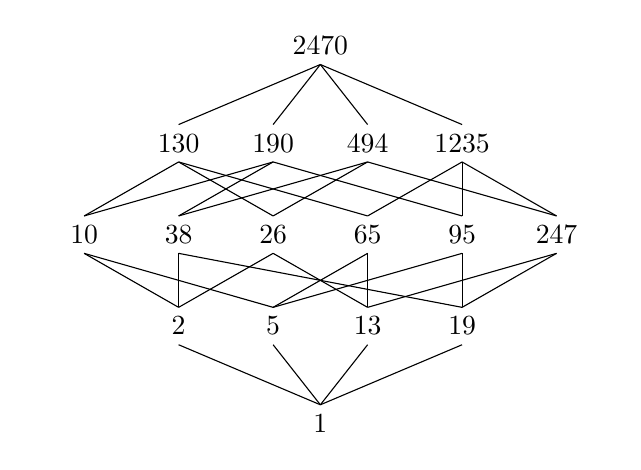
\begin{tikzpicture}
                % \hspace{-.3cm}
                \matrix (A) [matrix of nodes, row sep=.7cm, nodes={minimum width=1.2cm}]
                {
                    \\
                         & $130$ & $190$ & $494$ & $1235$ &  \\
                    $10$ & $38$  & $26$  & $65$  & $95$   & $247$ \\
                         & $2$   & $5$   & $13$  & $19$   & \\
                };
                
                \node[above=1cm] at ($(A-2-3)!0.5!(A-2-4)$) (top) {$2470$};
                \foreach \i in {2,...,5}
                \draw (top.south) -- (A-2-\i.north);
                
                \foreach \i/\j in {1/1, 1/3, 1/4, 2/1, 2/2, 2/5, 3/2, 3/3, 3/6, 4/4, 4/5, 4/6}
                    \pgfmathsetmacro{\i}{int(\i+1)}
                    \draw (A-2-\i.south)--(A-3-\j.north);
                
                \foreach \i/\j in {1/1, 1/2, 2/1, 2/4, 3/1, 3/3, 4/2, 4/3, 5/2, 5/4, 6/3, 6/4}
                \pgfmathsetmacro{\j}{int(\j+1)}
                \draw (A-3-\i.south)--(A-4-\j.north);
                
                \node[below=1cm] at ($(A-4-3)!0.5!(A-4-4)$) (bottom) {$1$};
                \foreach \i in {2,...,5}
                \draw (A-4-\i.south)--(bottom.north);
            \end{tikzpicture}
            }
            \caption{Hasse diagram of the poset $(D_{2470}, \mid)$}
            \label{fig:Q2a}
        \end{subfigure}
        \begin{subfigure}{0.49\textwidth}
            {\scriptsize
            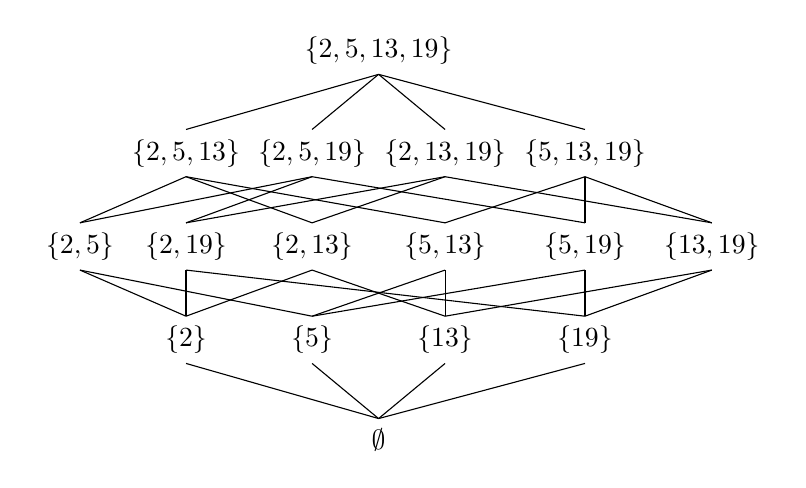
\begin{tikzpicture}
                % \hspace{-.4cm}
                \matrix (A) [matrix of nodes, row sep=.6cm, nodes={minimum width=1cm}]
                {
                    \\
                    & $\{2, 5, 13\}$ & $\{2, 5, 19\}$ & $\{2, 13, 19\}$ & $\{5, 13, 19\}$ &  \\
                    $\{2, 5\}$ & $\{2, 19\}$ & $\{2, 13\}$ & $\{5, 13\}$ & $\{5, 19\}$ & $\{13, 19\}$ \\
                    & $\{2\}$ & $\{5\}$ & $\{13\}$ & $\{19\}$ & \\
                };
                
                \node[above=1cm] at ($(A-2-3)!0.5!(A-2-4)$) (top) {$\{2, 5, 13, 19\}$};
                \foreach \i in {2,...,5}
                \draw (top.south) -- (A-2-\i.north);
                
                \foreach \i/\j in {1/1, 1/3, 1/4, 2/1, 2/2, 2/5, 3/2, 3/3, 3/6, 4/4, 4/5, 4/6}
                    \pgfmathsetmacro{\i}{int(\i+1)}
                    \draw (A-2-\i.south)--(A-3-\j.north);
                
                \foreach \i/\j in {1/1, 1/2, 2/1, 2/4, 3/1, 3/3, 4/2, 4/3, 5/2, 5/4, 6/3, 6/4}
                \pgfmathsetmacro{\j}{int(\j+1)}
                \draw (A-3-\i.south)--(A-4-\j.north);
                
                \node[below=1cm] at ($(A-4-3)!0.5!(A-4-4)$) (bottom) {$\emptyset$};
                \foreach \i in {2,...,5}
                \draw (A-4-\i.south)--(bottom.north);
            \end{tikzpicture}
            }
            \caption{Hasse diagram of the poset $(\mathcal{P}(\{2, 5, 19, 13\}), \subseteq)$}
            \label{fig:Q2b}
        \end{subfigure}
        \caption{Two isomorphic Hasse diagrams.}
        \label{fig:Q2}
    \end{figure}

\subsection*{\Exercise}
    A binary tree is a structure in which each node in the tree has at most two children nodes branching off of it, as shown in Figure \ref{fig:Q3}. A binary tree is \textit{full} if all of its nodes have either zero or two children. Let $B_{n}$ denote the number of full binary trees with $n$ nodes.
    
    \vspace{1.5mm}
    For $n > 1$, give a recurrence relation for $B_{n}$ (You do not have to find a closed form). Justify your answer.

    \begin{figure}[htbp]
        \centering
        \begin{subfigure}{.4\textwidth}
            \centering
            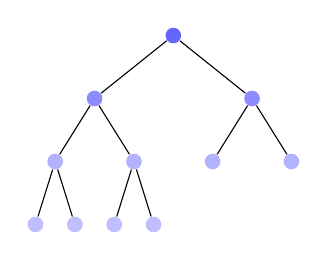
\begin{tikzpicture}
                [level distance=8mm,
                every node/.style={fill=blue!60,circle,inner sep=2pt},
                level 1/.style={sibling distance=20mm,nodes={fill=blue!45}},
                level 2/.style={sibling distance=10mm,nodes={fill=blue!30}},
                level 3/.style={sibling distance=5mm,nodes={fill=blue!25}}]
                \node {}
                child {node {}
                child {node {}
                child {node {}}
                child {node {}}
                }
                child {node {}
                child {node {}}
                child {node {}}
                }
                }
                child {node {}
                child {node {}
                }
                child {node {}}
                };
            \end{tikzpicture}
        \end{subfigure}
        \begin{subfigure}{.4\textwidth}
            \centering
            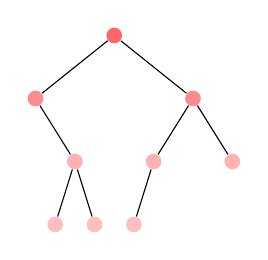
\begin{tikzpicture}
                [level distance=8mm,
                every node/.style={fill=red!60,circle,inner sep=2pt},
                level 1/.style={sibling distance=20mm,nodes={fill=red!45}},
                level 2/.style={sibling distance=10mm,nodes={fill=red!30}},
                level 3/.style={sibling distance=5mm,nodes={fill=red!25}}]
                \node {}
                child {node {}
                child[missing]
                child {node {}
                child {node {}}
                child {node {}}
                }
                }
                child {node {}
                child {node {}
                child {node {}}
                child[missing]
                }
                child {node {}}
                };
            \end{tikzpicture}
        \end{subfigure}
        \caption{Two examples of binary trees. The tree on the left is full, while the tree on the right is not.}
        \label{fig:Q3}
    \end{figure}

\subsection*{Solution}
    Suppose we have $B_{1}, B_{2}, \dots, B_{n - 1}$, and we wish to find $B_{n}$. To do this, note that any full binary tree will have a root node. For $n > 1$, this root node is guaranteed to have two children, and thus two child trees. The left child tree can have anywhere from $1 \le i \le n - 2$ nodes. The right child tree will have a corresponding $n - 1 - i$ nodes. Summing all possibilities of $i$ gives us the recurrence relation $B_{n}$: $$B_{n} = \sum_{i = 1}^{n - 2} B_{i}B_{n - 1 - i}.$$
    This recurrence relation is satisfied with the base cases $B_{1} = 1$ and $B_{2} = 0$.

\subsection*{\Exercise}
    Use the method of your choice to solve the following recursions.
    \begin{enumerate}
        \item $T(n) = 5T(n - 1) - 8T(n - 2) + 4T(n - 3) \text{ where $T(0) = 1$, $T(1) = 0$, and $T(2) = 0$}.$
        \item $T(n) = 2T(n/2) + n\log(n) \text{ where } T(1) = c \text{ (here $c$ is a constant)}.$
    \end{enumerate}
    {\small Note: While you may use any of the methods discussed in class to solve these recurrences, in each part, there may be a method considered ``easier" than the other.}

\subsection*{Solution}
    \begin{enumerate}
        \item \textit{(Substitution Method)} Using repeated substitutions, we have 
        \begin{align*}
            T(0) &= 1 = (0 - 3)2^{0} + 4, \\
            T(1) &= 0 = (1 - 3)2^{1} + 4, \\
            T(2) &= 0 = (2 - 3)2^{2} + 4, \\
            T(3) &= 5T(2) - 8T(1) + 4T(0) = 4 = (3 - 3)2^{3} + 4, \\
            T(4) &= 5T(3) - 8T(2) + 4T(1) = 20 = (4 - 3)2^{4} + 4, \\
            T(5) &= 5T(4) - 8T(3) + 4T(2) = 68 = (5 - 3)2^{5} + 4, \\
            &\vdotswithin{ = } \\
            T(n) &= 5T(n - 1) - 8T(n - 2) + 4T(n - 3) = (n - 3)2^{n} + 4.
        \end{align*}
        We prove the $n^{th}$-term guess by mathematical induction. Let $P(n)$ be the sentence $$T(n) = (n - 3)2^{n} + 4.$$
        \textsc{Base Case}: $P(0)$, $P(1)$, and $P(2)$ are all true, since
        \begin{align*}
            T(0) &= 1 = (0 - 3)2^{0} + 4, \\
            T(1) &= 0 = (1 - 3))2^{1} + 4, \\
            T(2) &= 0 = (2 - 3)2^{2} + 4.
        \end{align*}
        \textsc{Inductive Step}: Now let $n \ge 0$ such that $P(n)$, $P(n + 1$, and $P(n + 2)$ are all true. Then 
        $$\begin{aligned}
            T(n + 3) &= 5T(n + 2) - 8T(n + 1) + 4T(n) \\
            &= 5((n - 1)2^{n + 2} + 4) - 8((n - 2)2^{n + 1} + 4) + 4((n - 3)2^{n} + 4) \\
            &= (5n - 5)2^{n + 2} - (4n - 8)2^{n + 2} + (n - 3)2^{n + 2} + 20 - 32 + 16 \\
            &= n \cdot 2^{n + 3} + 4.
        \end{aligned}$$
        Hence $P(n + 3)$ is true as well. \\
        \textsc{Conclusion}: Therefore by strong induction, for all $n \ge 0$, $P(n)$ is true.
        \item \textit{(Iteration Method)} Note that 
        $$\begin{aligned}[t]
            T(n) &= 2T(\tfrac{n}{2}) + n \log(n) \\
            &= 2(2T(\tfrac{n}{2^2}) + \tfrac{n}{2}\log(\tfrac{n}{2})) + n\log(n) \\
            &= 2^{2}T(\tfrac{n}{2^{2}}) + n(\log(n) - \log(2)) + n\log(n) \\
            &= 2^{2}T(\tfrac{n}{2^{2}}) + 2n\log(n) - n \\
            &= 2^{3}T(\tfrac{n}{2^{3}}) + 3n\log(n) - n - 2n \\
            &\vdotswithin{ = } \\
            &= 2^{k}T(\tfrac{n}{2^{k}}) + kn \log(n) - n\textstyle\sum_{i = 1}^{k - 1} i \\
            &= 2^{k}T(\tfrac{n}{2^{k}}) + kn \log(n) - \tfrac{n}{2}(k - 1)k.
        \end{aligned}$$
        Let $k = \log n$, then $n = 2^{k}$ and  $$T(n) = nT(1) + n\log^{2}(n) - \tfrac{n}{2}(\log(n) - 1)\log(n) = cn + \tfrac{1}{2}n \log^{2}n + \tfrac{1}{2}n\log{n}.$$
    \end{enumerate}

\subsection*{\Exercise}
    In each part, as in lecture, start with the definition and get the values of $c$ and $k$.
    \begin{enumerate}
        \item Let $f_{1}, f_{2}, g$ be real functions satisfying $f_{1} = O(g_{1})$ and $f_{2} = O(g_{2})$. Also let $a \in \mathbb{R}$. Show that $a \cdot f = O(g)$ for all $a \in \mathbb{R}^{*}$.
        \item Let $f_{1}, f_{2}, g$ be real functions satisfying $f_{1} = O(g)$ and $f_{2} = O(g)$ Show that $f_{1} + f_{2} = O(g)$.
        \item Let $f_{1}, f_{2}, g_{1}, g_{2}$ be real functions satisfying $f_{1} = O(g_{1})$ and $f_{2} = O(g_{2})$. Show that $f_{1} \cdot f_{2} = O(g_{1} \cdot g_{2})$.
    \end{enumerate}

\subsection*{Solution}
    \begin{enumerate}
        \item Since $f_{1} = O(g)$, there exists some $k, c_{0} > 0$ such that $|f(x)| < c_{0}|g(x)|$ for all $x > k$. Choosing $c = |a|c_{0}$, we have that $|af(x)| < c|g(x)|$ for all $x > k$ and $a \in \mathbb{R}^{*}$. Hence $a \cdot f = O(g)$.
        \item Since $f_{1} = O(g)$, there exists some $k_1, c_1 > 0$ such that $|f_{1}(x)| < c_{1}|g(x)|$ for all $x > k_{1}$. Since $f_{2} = O(g)$, there exists some $k_2, c_2 > 0$ such that $|f_{2}(x)| < c_{2}|g(x)|$ for all $x > k_{2}$. Choosing $k = \max(k_{1}, k_{2})$, we have that $|f_{1}(x) + f_{2}(x)| < |f_{1}(x)| + |f_{2}(x)| < (c_{1} + c_{2})|g(x)|$. Hence $f_{1} + f_{2} = O(g)$ for $c = c_{1} + c_{2}$ and $k = \max(k_{1}, k_{2})$.
        \item Since $f_{1} = O(g_{1})$, there exists some $k_1, c_1 > 0$ such that $|f_{1}(x)| < c_{1}|g_{1}(x)|$ for all $x > k_{1}$. Since $f_{2} = O(g_{2})$, there exists some $k_{2}, c_{2} > 0$ such that $|f_{2}(x)| < c_{2}|g_{2}(x)|$ for all $x > k_{2}$. Choosing $k = \max(k_{1}, k_{2})$, we have that $|f_{1}(x)f_{2}(x)| = |f_{1}(x)||f_{2}(x)| < c_{1}c_{2}|g_{1}(x)||g_{2}(x)| = c_{1}c_{2}|g_{1}(x)g_{2}(x)|$ for all $x > k$. Hence $f_{1}f_{2} = O(g_{1}g_{2})$ for $c = c_{1}c_{2}$ and $k = \max(k_{1}, k_{2})$.
    \end{enumerate}

\subsection*{\Exercise} % Next time, move  $n\log_{10}(n) + 1$ inside the log to n^n
    Let $A$ be the set of all functions $f: \mathbb{N}^{+} \rightarrow \mathbb{R}^{+}$. Consider the relation $\sim$ on $A$ defined as follows: $$\text{$f \sim g$ if there exist constants $c_{1}, c_{2} > 0$ such that $c_{1}g(n) < f(n) < c_{2}g(n)$ for all $n \in \mathbb{N}^{+}$.}$$
    \begin{enumerate}
        \item Show that $\sim$ is an equivalence relation.
        \item It can similarly be shown that $\Theta$ is an equivalence relation. Group the following functions by equivalence classes such that functions $f(n)$ and $g(n)$ are in the same equivalence class iff $f = \Theta(g)$ (you do not need to show your work): 
        \begin{multicols}{4}
        \begin{itemize}
            \item $\log_{2}(n) + 1$
            \item $\log_{16}(n!)$
            \item $2n + 5$
            \item $(\log_{2}(n))^{\log_{2}(n)}$
            \item $n\log_{10}(n) + 1$
            \item $2021n + \log_{10}(n)$
            \item $2^{n}$
            \item $n^{1/\log_{6}(n)}$
            \item $3^{n}$
            \item $\ln(n^{2}) + 2021$
            \item $\frac{8n^{2} + 3n + 9}{n^{2}}$
            \item $n^{\log_{2}(\log_{2}(n))}$
        \end{itemize}
        \end{multicols}
    \end{enumerate}

\subsection*{Solution}
    \begin{enumerate}
        \item $\sim$ is an equivalence relation iff it is reflexive, symmetric, and transitive. For any $f, g, h \in A$, we have
        \begin{enumerate}[label = \arabic*.]
            \item \textit{(Reflexivity)} Let $c_{1} = \frac{1}{2}$ and $c_{2} = 2$. Then $\frac{1}{2}f(n) < f(n) < 2f(n)$ for all $n \in \mathbb{N^{+}}$, so $f \sim f$.
            \item \textit{(Symmetry)} Suppose $f \sim g$. Then there exist constants $c_{1}, c_{2} > 0$ such that $c_{1}g(n) < f(n) < c_{2}g(n)$ for all $n \in \mathbb{N^{+}}$. Since $c_{1}, c_{2} > 0$, we can divide by $c_{1}$ and $c_{2}$ to obtain $\frac{1}{c_{2}}f(n) < g(n) < \frac{1}{c_{1}}f(n)$. Thus $g \sim f$.
            \item \textit{(Transitivity)} Suppose $f \sim g$ and $g \sim h$. Then there exist constants $c_{1}, c_{2}, c_{3}, c_{4} > 0$ such that $c_{1}g(n) < f(n) < c_{2}g(n)$ and $c_{3}h(n) < g(n) < c_{4}h(n)$ for all $n \in \mathbb{N^{+}}$. Substituting the inequalities for $g(n)$ found in the second equation into the first equation, we get that $c_{1}c_{3}h(n) < f(n) < c_{2}c_{4}h(n)$. Thus $f \sim h$.
        \end{enumerate}
        \item The equivalence classes of these functions are
        \begin{gather*}
            \{2n + 5, 2021n + \log_{10}(n)\}, \\
            \{\log_{2}(n) + 1, \ln(n^{2}) + 2021\}, \\
            \{n^{1/\log_{6}(n)}, \textstyle \frac{8n^{2} + 3n + 9}{n^{2}}\}, \\
            \{n^{\log_{2}(\log_{2}(n))}, (\log_{2}(n))^{\log_{2}(n)}\}, \\
            \{\log_{16}(n!), n\log_{10}(n) + 1\}, \\
            \{2^{n}\}, \text{ and } \{3^{n}\}.
        \end{gather*} 
        Brief informal explanations for each of the equivalence classes are shown below.
        \begin{itemize}
            \item $2n + 5 = \Theta(2021n + \log_{10}(n))$, since $\log_{10}(n) = \mathcal{O}(n)$.
            \item $\log_{2}(n) + 1 = \Theta(\ln(n^{2}) + 2021)$, since $\ln(n^{2}) = 2\ln(n) = \frac{2}{\log_{2}(e)}\log_{2}{n}$.
            \item $n^{1/\log_{6}(n)} = \Theta(\frac{8n^{2} + 3n + 9}{n^{2}})$, since $n^{1/\log_{6}(n)} = n^{\log_{6}(6) / \log_{6}(n)} = n^{\log_{n}(6)} = 6$.
            \item $n^{\log_{2}(\log_{2}(n))} = (2^{\log_{2}(n)})^{\log_{2}(\log_{2}(n))} = (2^{\log_{2}(\log_{2}(n))})^{\log_{2}(n)} = (\log_{2}(n))^{\log_{2}(n)}$.
            \item $\log_{16}(n!) = \Theta(n\log_{10}(n) + 1)$. It is sufficient to demonstrate that $\log_{16}(n!) = \mathcal{O}(n\log_{16}(n) + 1)$ and $\log_{16}(n!) = \Omega(n\log_{16}(n) + 1)$.
            \begin{itemize}
                \item $\log_{16}(n!) = \log_{16}(n \cdot (n - 1) \cdot \dots \cdot 1) = \log_{16}(n) + \log_{16}(n - 1) + \dots + \log_{16}(1) \le n\log_{16}(n)$
                \item
                $\begin{aligned}[t]
                    \log_{16}(n!) = \log_{16}(n \cdot (n - 1) \cdot \dots \cdot 1) &= \log_{16}(1) + \log_{16}(2) + \dots + \log_{16}(n)  \\
                    &\textstyle \ge \log_{16}(\frac{n}{2}) + \log_{16}(\frac{n}{2} + 1) + \dots + \log_{16}(n) \\
                    &\textstyle \ge \frac{1}{2}n\log_{16}(n)
                \end{aligned}$
            \end{itemize}
            \item Finally, note that while $\log_{x}(2^{n}) = \Theta(\log_{x}(3^{n}))$ for any $x$, $2^{n} \ne \Theta(3^{n})$. This can be seen through contradiction, as if $2^{n} = \Theta(3^{n})$, then for some $n \ge n_{0}$, there exists a constant $c$ such that $$3^{n} = (2 \times 1.5)^{n} = 2^{n} \times 1.5^{n} = c \cdot 2^{n} \implies c = 1.5^{n}.$$ But there is no constant $c$ satisfying this condition.
        \end{itemize}
    \end{enumerate}

\subsection*{\Exercise}
    \textit{(For this problem, you can use classical tools from Calculus such as $\epsilon-\delta$ definition of limits, derivatives, etc.)} Let $f, g$ be real functions with $f$ not identically zero and $g(x) \ne 0$ for all $x \in \mathbb{R}$ satisfying $$\lim_{x \rightarrow \infty} \left|\frac{f(x)}{g(x)}\right| = \ell.$$
    \begin{enumerate}
        \item Show that if $0 < \ell < \infty$, then $f = \Theta(g)$.
        \item Show that, if $l = 0$, then $f = \mathcal{O}(g)$. Give an example of functions for which $g \ne \mathcal{O}(f)$.
        \item Can you deduce a relation (of the form big-$\mathcal{O}$, big-$\Omega$, or big-$\Theta$) between $f$ and $g$ if $\ell = \infty$? Prove your answer.
        \item Let $p(x) = a_{n}x^{n} + a_{n - 1}x^{n - 1} + \dots + a_{1}x + a_{0}$ and $q(x) = b_{m}x^{m} + b_{m - 1}x^{m - 1} + \dots + b_{1}x + b_{0}$ be two polynomials with real coefficients. Use parts (a)--(c) to deduce when $p = \mathcal{O}(q)$, $p = \Omega(q)$, or $p = \Theta(q)$ \textit{(your answer should depend on $n$ and $m$)}.
    \end{enumerate}

\subsection*{Solution}
    \begin{enumerate}
        \item Suppose $0 < \ell < \infty$. Then by the formal definition of the limit, for all $\epsilon > 0$, there exists some $k > 0$ such that for all $x > k$, $\left|\left|\frac{f(x)}{g(x)}\right| - \ell\right| < \epsilon$. Now
        \begin{align*}
            \left|\left|\frac{f(x)}{g(x)}\right| - \ell\right| < \epsilon &\iff - \epsilon < \left|\frac{f(x)}{g(x)}\right| - \ell < \epsilon \\
            &\iff \ell - \epsilon < \frac{|f(x)|}{|g(x)|} < \ell + \epsilon \\
            &\iff (\ell - \epsilon)\left|g(x)\right| < \left|f(x)\right| < (\ell + \epsilon)\left|g(x)\right|.
        \end{align*}
        Since this statement is true for all $\epsilon > 0$, we can use universal instantiation to conclude that this statement is true for some $0 < \epsilon < l$. Thus there exists some $c_{1} = \ell - \epsilon > 0$, some $c_{2} = \ell + \epsilon > 0$, and some $k > 0$ such that $c_{1}|g(x)| < |f(x)| < c_{2}|g(x)|$ for all $x > k$, and so $f = \Theta(g)$.
        \item Suppose $\ell = 0$. Then again using the formal definition of the limit, we have that for some $c = \epsilon > 0$ and some $k > 0$ such that $|f(x)| < c|g(x)|$ for all $x > k$. Hence $f = \mathcal{O}(g)$.
        
        \vspace{1.5mm}
        However, $g \ne \mathcal{O}(f)$. To see this, take $f(x) = x$ and $g(x) = x^2$.
        \item Suppose $l = \infty$. By the formal definition of the limit, this means that for all $c > 0$, there exists some $k > 0$ such that for all $x > k$, $\left|\frac{f(x)}{g(x)}\right| > c$. Again using universal instantiation, we conclude that there exists some $c, k > 0$ such that $c|g(x)| < |f(x)|$ for all $x > k$. Hence $f = \Omega(g)$.
        \item The three cases below are disjoint and cover all possibilities for $n$ and $m$.
        \begin{align*}
            n > m &\iff \lim_{x \rightarrow \infty} \left|\frac{p(x)}{q(x)}\right| = \infty \implies p = \Omega(q) \\
            m > n &\iff \lim_{x \rightarrow \infty} \left|\frac{p(x)}{q(x)}\right| = 0 \implies p = \mathcal{O}(q) \\
            m = n &\iff \lim_{x \rightarrow \infty} \left|\frac{p(x)}{q(x)}\right| = \frac{b_{m}}{a_{n}} \implies p = \Theta(q)
        \end{align*}
    \end{enumerate}

\end{document}
